\documentclass[tikz,border=2pt]{standalone}
\usepackage{amsmath,amssymb,mathtools}
\usepackage{pgfplots}
\pgfplotsset{compat=1.18}
\usetikzlibrary{arrows.meta}

\begin{document}
% f(x) = e^{-1/x} for x > 0 and 0 for x <= 0 is infinitely differentiable, all its derivatives
% vanish at 0, so its Taylor series at 0 is 0; but f is not 0 for x > 0: not real analytic at 0.
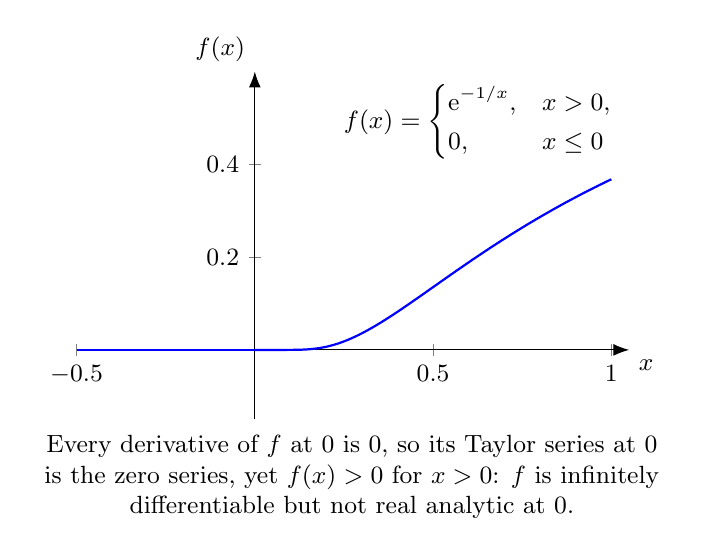
\begin{tikzpicture}[every node/.style={font=\small}]
	\begin{axis}[
		width=8.6cm, height=6cm,
		axis lines=middle, axis line style={-{Latex[length=2mm]}},
		xmin=-0.5, xmax=1.05, ymin=-0.15, ymax=0.6,
		xtick={-0.5,0.5,1}, ytick={0.2,0.4},
		tick label style={font=\small},
		xlabel={$x$}, ylabel={$f(x)$},
		xlabel style={below right}, ylabel style={above left},
		clip=false
		]
		\addplot[blue, thick, domain=-0.5:0] {0};
		\addplot[blue, thick, domain=0.001:1, samples=200] {exp(-1/x)};
		\node[anchor=north east] at (axis description cs:0.99,0.99) {$f(x)=\begin{dcases}\mathrm{e}^{-1/x}, & x>0,\\ 0, & x\le0\end{dcases}$};
	\end{axis}
	\node[anchor=north, align=flush center, text width=8cm] at ([yshift=-2pt]current axis.outer south) {Every derivative of $f$ at $0$ is $0$, so its Taylor series at $0$ is the zero series, yet $f(x)>0$ for $x>0$: $f$ is infinitely differentiable but not real analytic at $0$.};
\end{tikzpicture}
\end{document}
